\documentclass{article}

\usepackage[romanian]{babel}
\usepackage{amsmath}
\usepackage{indentfirst} % indenteaza primul paragraf din fiecare sectiune
\usepackage{graphicx}
\usepackage{caption}
\usepackage{hyperref}

\title{Referat: Termistorul \\ \large Studiul Variației Rezistenței Electrice cu
	Temperatura la Materiale Semiconductoare}
\author{Nicolas Dumitru}

\begin{document}

\maketitle

\section{Scopul lucrării}
Vom verifica legea dependenței în funcție de temperatură a rezistenței electrice
a materialelor semiconductoare.

\section{Teoria lucrării}
Energia Fermi a materialelor semiconductoare pure/slab dopate se află în banda
interzisă la temperaturi mai mici de câteva sute de grade Celsius.

Pentru $T \neq 0$, banda de conducție va fi populată de agitația termică cu o
concentrație de electroni liberi notată $n$, iar în banda de valență vor apărea
goluri în concentrație $p$.

Pentru semiconductori nedopați, avem $p = n$.

Teoria benzilor de energie în materialele semiconductoare ne dă expresiile celor
două concentrații de sarcini electrice:
\begin{align}
	n & = 2(2 \pi m_e k T)^{\frac{3}{2}} \cdot h^{-3} \cdot
	\exp\left( -\frac{E_c - E_F}{kT} \right)
	\label{eq:concentratie_n}                               \\
	p & = 2(2 \pi m_g k T)^{\frac{3}{2}} \cdot h^{-3} \cdot
	\exp\left( -\frac{E_F - E_v}{kT} \right)
	\label{eq:goluri_p}
\end{align}
\begin{flalign*}
	m_e & = \text{masa efectivă a electronilor}                          &  & \\
	m_g & = \text{masa efectivă a golurilor}                             &  & \\
	k   & = \text{constanta Boltzmann}                                   &  & \\
	h   & = \text{constanta Planck}                                      &  & \\
	E_c & = \text{energia corespunzătoare minimului benzii de conducție} &  & \\
	E_v & = \text{energia corespunzătoare plafonului benzii de valență}  &  & \\
	E_F & = \text{energia nivelului Fermi aflat}
\end{flalign*} % evităm un warning (misterios) lăsînd un rînd liber

În cazul semiconductorilor intrinseci, avem $E_F = \frac{E_c + E_v}{2}$ (la
jumătatea "distanței" dintre $E_c$ și $E_v$). % TODO: check; am inteles bine?

\begin{equation}
	\eqref{eq:concentratie_n} \land \eqref{eq:goluri_p} \implies
	n \cdot p = A \exp\left( - \frac{E_c - E_v}{kT} \right)
\end{equation}

\begin{equation}
	n = p = n_i \label{eq:n_p}
\end{equation}

\begin{equation}
	\eqref{eq:concentratie_n} \land \eqref{eq:goluri_p} \land \eqref{eq:n_p}
	\implies n_i = B \exp\left( - \frac{E_c - E_v}{2kT} \right)
\end{equation}

Conductibilitatea electrică a unui semiconductor este:
\begin{equation}
	\sigma = \frac{1}{\rho} = e(n\mu_n + p\mu_p)
\end{equation}

$\Delta E = E_c - E_v$ este lărgimea benzii (zonei) interzise.

Mobilitățile $\mu_n$ și $\mu_p$ fiind practic independente de temperaturå, avem:
\begin{equation}
	\begin{aligned}
		\sigma & \propto \exp\left( - \frac{E_c - E_v}{2kT} \right) \\
		\rho   & \propto \exp\left( \Delta E / 2kT \right)
		\text{.}
	\end{aligned}
\end{equation}

Rezistența unei probe semiconductoare este dată de ecuația
\begin{equation}
	R = C \exp\left( \frac{\Delta E}{2kT} \right)
	\label{eq:rezistenta}
\end{equation}
și ilustrată în Figura \ref{fig:grafic_RT}.

\begin{figure}[htbp]
	\centering
	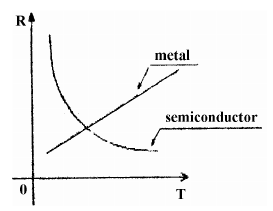
\includegraphics[width=0.6\textwidth]{rez-temp.png}
	\caption{Dependența rezistenței de temperatură}
	\label{fig:grafic_RT}
\end{figure}

Prin logaritmare expresiei \eqref{eq:rezistenta}, obținem
\begin{equation}
	\ln R = C + \frac{\Delta E}{2kT}
	\text{.}
\end{equation}

\section{Schițe}
\begin{figure}[htbp]
	\centering
	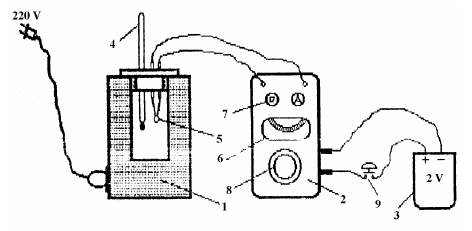
\includegraphics[width=0.6\textwidth]{device.png}
	\caption{Dependența rezistenței de temperatură}
	\label{fig:device}
\end{figure}

\end{document}
